\chapter{Atención}
Como se ha descrito en el capítulo anterior, antes de la popularización del mecanismo de \textit{atención} la mayoría de modelos para el procesamiento de lenguaje natural disponían de un componente, el \textit{codificador}, que codificaba la secuencia de entrada de longitud variable en un \textit{estado}, una representación de la entrada de longitud fija y de un segundo componente, el \textit{decodificador}, que actuaba como un modelo condicional del lenguaje, prediciendo cada símbolo de salida a partir del estado y los símbolos ya generados.

El mecanismo de atención hereda la distinción entre \textit{codificador} y \textit{decodificador}, pero parte de la idea de que el decodificador revisite la entrada a cada paso de forma que, en lugar de ver siempre la misma representación, pueda prestar atención de forma dinámica a distintas partes de la entrada. Diseñando el mecanismo de atención como una función diferenciable, el problema de a qué partes de la entrada debe prestar atención puede resolverse como un problema de optimización usando, por ejemplo, descenso de gradiente. En este capítulo se formaliza la noción de atención y se discuten algunas de sus variantes.

\section{Atención}

\begin{definition}[Base de datos]
    Sean \( d_k, d_v \in \nat \) y dos sucesiones \( \Set{ k_n }_{n = 1}^N \) con \( k_n \in \real{d_k} \), \( \Set{v_n}_{n = 1}^N \) con  \( v_n \in \real{d_v} \), que llamaremos \textit{claves} y \textit{valores} respectivamente. Llamamos \textit{base de datos} al conjunto ordenado \( \mathcal{D} = \left\{ (k_n, v_n) \colon n = 1, …, N \right\} \),
\end{definition}

\begin{definition}[Atención] Sea \( \mathcal{D} = \Set{(k_n, v_n) \colon n = 1, …, N} \) una base de datos con \( k_n \in \real{d_k}, v_n \in \real{d_v}\). Dado un vector \( q \in \real{d_q} \) (llamado consulta o \textit{query}) y una función \( \alpha \colon \real{d_q} \times \real{d_k} \to \realo \) definimos la \textit{atención de \( q \) sobre \( \mathcal{D} \)} como:
\[
\attention(q, \mathcal{D}; \alpha) = \sum^N_{n = 1} \alpha(q, k_n) v_n
\]
\end{definition}

Los coeficientes \( \alpha(q, k_n) \) determinan la ponderación de cada valor de la base de datos. La función \( \alpha \) recibe el nombre de función o \textit{kernel} de similitud, pues por lo general asigna una mayor ponderación a los valores asociados a las claves más similares a la consulta.

Es común imponer las condiciones \( \sum_n \alpha(q, k_n) = 1 \), \( \alpha(q, k_n) \geq 0\) de forma que el vector de atención sea una combinación convexa de los valores.

\section{El estimador de Nadaraya-Watson}
Presentamos a continuación un ejemplo del mecanismo de atención aplicado a problemas de regresión: el estimador de Nadaraya-Watson \cite{watson1964smooth,nadaraya1964estimating}.

Nos encontramos en el marco habitual de un problema de regresión: disponemos de un conjunto de carácterísticas observadas \( \Set{x_{n}}_{n = 1}^N \) con \( x_{n}  \in \real{k} \) y una sucesión \( \Set{y_n}_{n = 1}^N \) con \( y_n \in \realo \) que recoge el valor de la variable objetivo para cada una de las observaciones. Dada una nueva observación \( x_{0} \), queremos aproximar el valor de la variable objetivo \( y_{0} \) mediante un estimador \( \widehat{y}_{0} \).

Definimos la base de datos \( \mathcal{D} = \Set{ (x_{n}, y_{n}) \colon n = 1, \dots, N } \). Dada una función de similitud  \( \alpha : \real{k} \times \real{k} \to \realo \), la atención de \( q \) sobre \( \mathcal{D} \) es:
\[
    \attention(q, \mathcal{D}; \alpha) = \sum_n \alpha(q, x_{n}) y_{n}
\]
y podemos aproximar \( y_{0} \) mediante el estimador
\begin{equation}\label{eq:kde}
    \widehat{y}_{0} = \attention(x_{0}, \mathcal{D}; \alpha) 
\end{equation}

Por conveniencia, asumiremos que \( \alpha \) es una función normalizada entre \( 0 \) y \( 1 \), de la forma:
\[
    \alpha(q, x_n) = \frac{a(q, x_n)}{\sum_i a(q, x_{i}) }
\]
para alguna función \( a : \real{k} \times \real{k} \to \realo \).

La \cref{fig:regression} muestra el resultado de estimar la distribución de \( N = 50 \) puntos de la forma \( \Set{(x_{n}, y_{n})}_{n = 1}^N \) siendo \( \Set{x_{n}} \) un conjunto ordenado de puntos del intervalo \( [0, 10] \) escogidos aleatoriamente (con probabilidad uniforme) e \( \Set{y_n} \) de la forma: 
\[
    y_{n} = x_{n} + \sin(x_{n}) + \epsilon \quad \text{ con \( \epsilon \sim \mathcal{N}(0, 1)\)}
\]
La estimación se realiza sobre una partición equiespaciada \( \Set{x^\text{val}_{i}} \) de \( [0, 10] \) formada por 50 puntos, utilizando la \cref{eq:kde} y varios \textit{kernel} de similitud distintos para estimar \( \Set{\widehat{y}^\text{val}_{i}} \):
\[
    \begin{split}\begin{aligned}
    a(q, k) & = \exp\left(-\frac{1}{2} \|q - k\|^2 \right) && \mathrm{Gaussiana} \\
    a(q, k) & = \max\left(0, 1 - \|q - k\|\right) && \mathrm{Epanechikov} \\
    a(q, k) & = \begin{cases}
        1 &\text{ si } \|q - k\| \leq 1 \\
        0 &\text{ si no}
    \end{cases} && \mathrm{Boxcar}
    \end{aligned}\end{split}
\]

La estimación es notablemente precisa, aunque la suavidad de la estimación depende del tipo concreto de \textit{kernel} escogido. La \cref{fig:kernel} muestra una visualización de los pesos de atención: observamos que las magnitudes mayores se concentran en torno a la diagonal, dado que \( x^\text{val}_{i} \simeq x_j \) para índices \( i, j \) cercanos. 

\begin{figure}[tb]
    \centering
    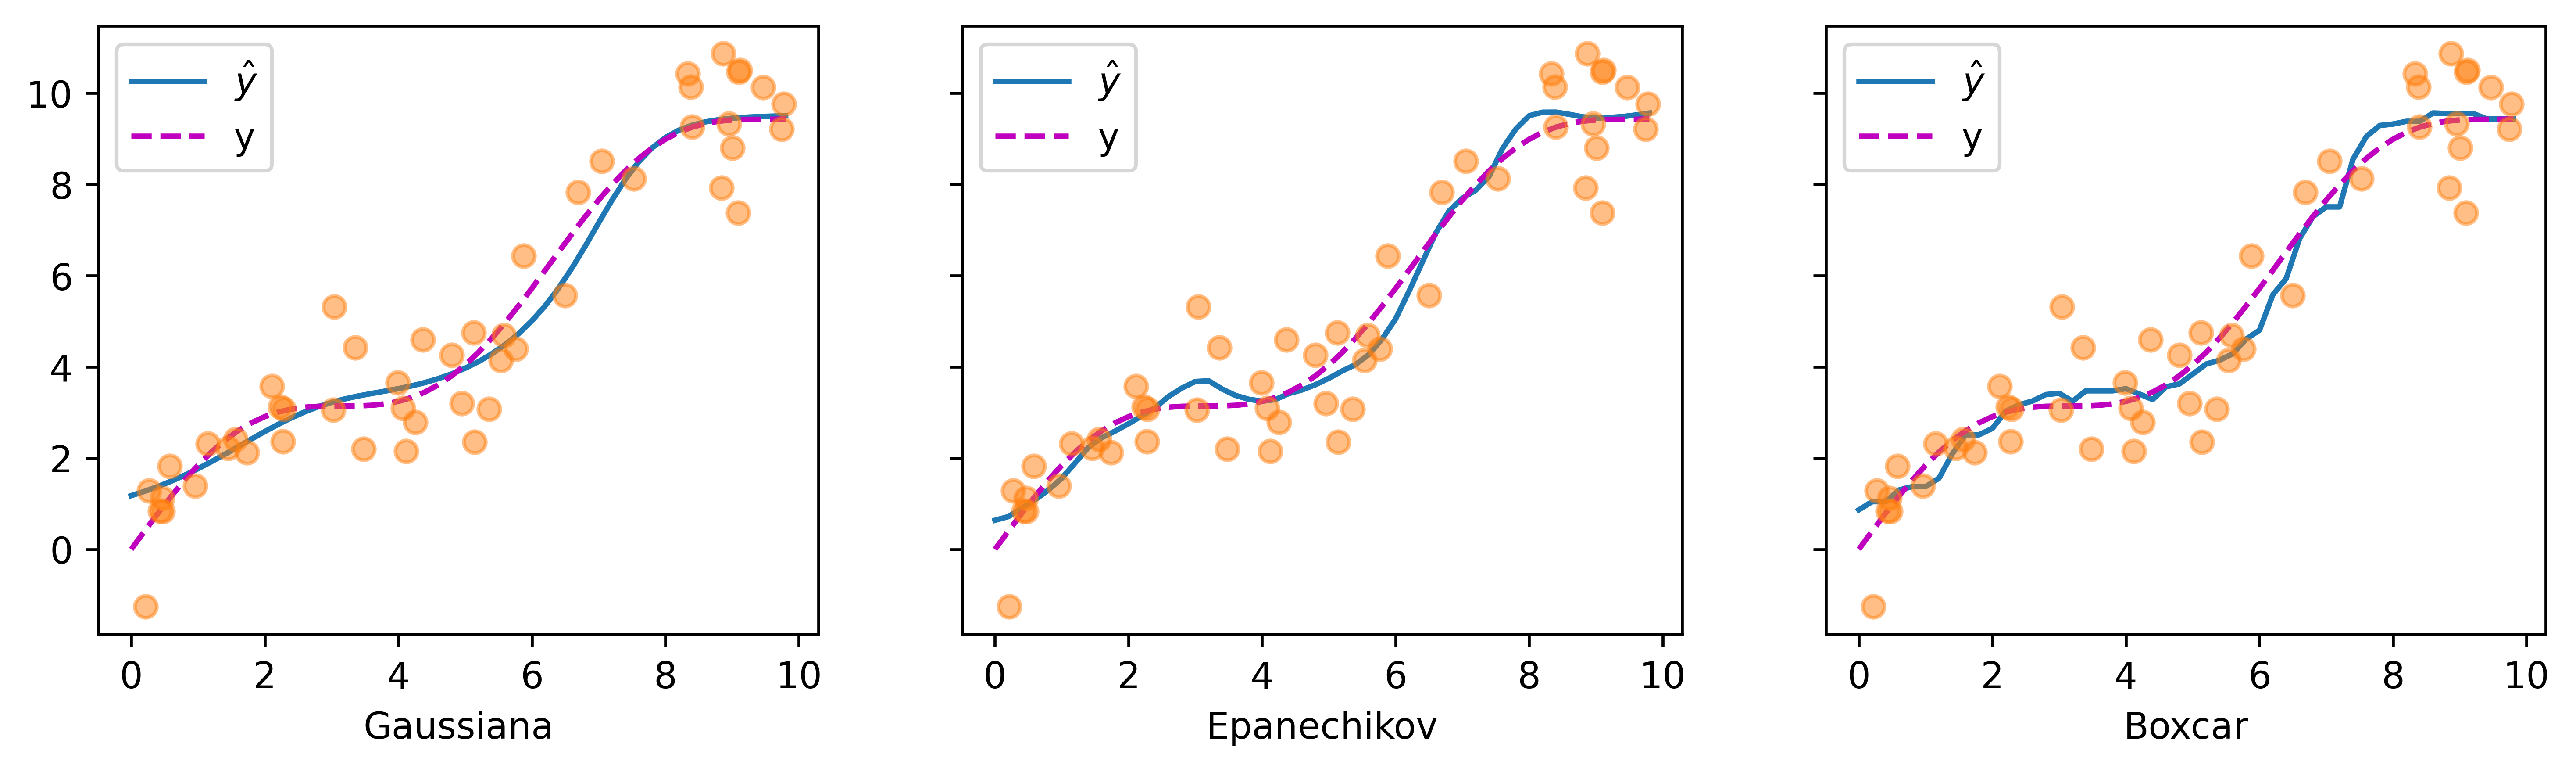
\includegraphics[width=\textwidth]{figures/chapter4/graph.png}
    \caption{Estimación de la función \( y \) mediante la estimación del valor de la variable objetivo sobre una partición equiespaciada del intervalo \( [0, 10] \) usando tres kérneles de similitud distintos.}
    \label{fig:regression}
\end{figure}

Esta forma de utilizar la atención es una forma de \textit{estimación de densidad de kernel}, una técnica clásica de inferencia no paramétrica que tiene la ventaja de que no requiere de ningún entrenamiento. Existen diversas heurísticas para elegir el \textit{kernel} \cite{silverman1986density} y puede probarse que si la anchura del \textit{kernel} se ajusta adecuadamente conforme se añaden observaciones entonces el método converge al valor real \( \E \llbracket y | x \rrbracket \) \cite{mack1982weak}.

\begin{figure}[tb]
    \centering
    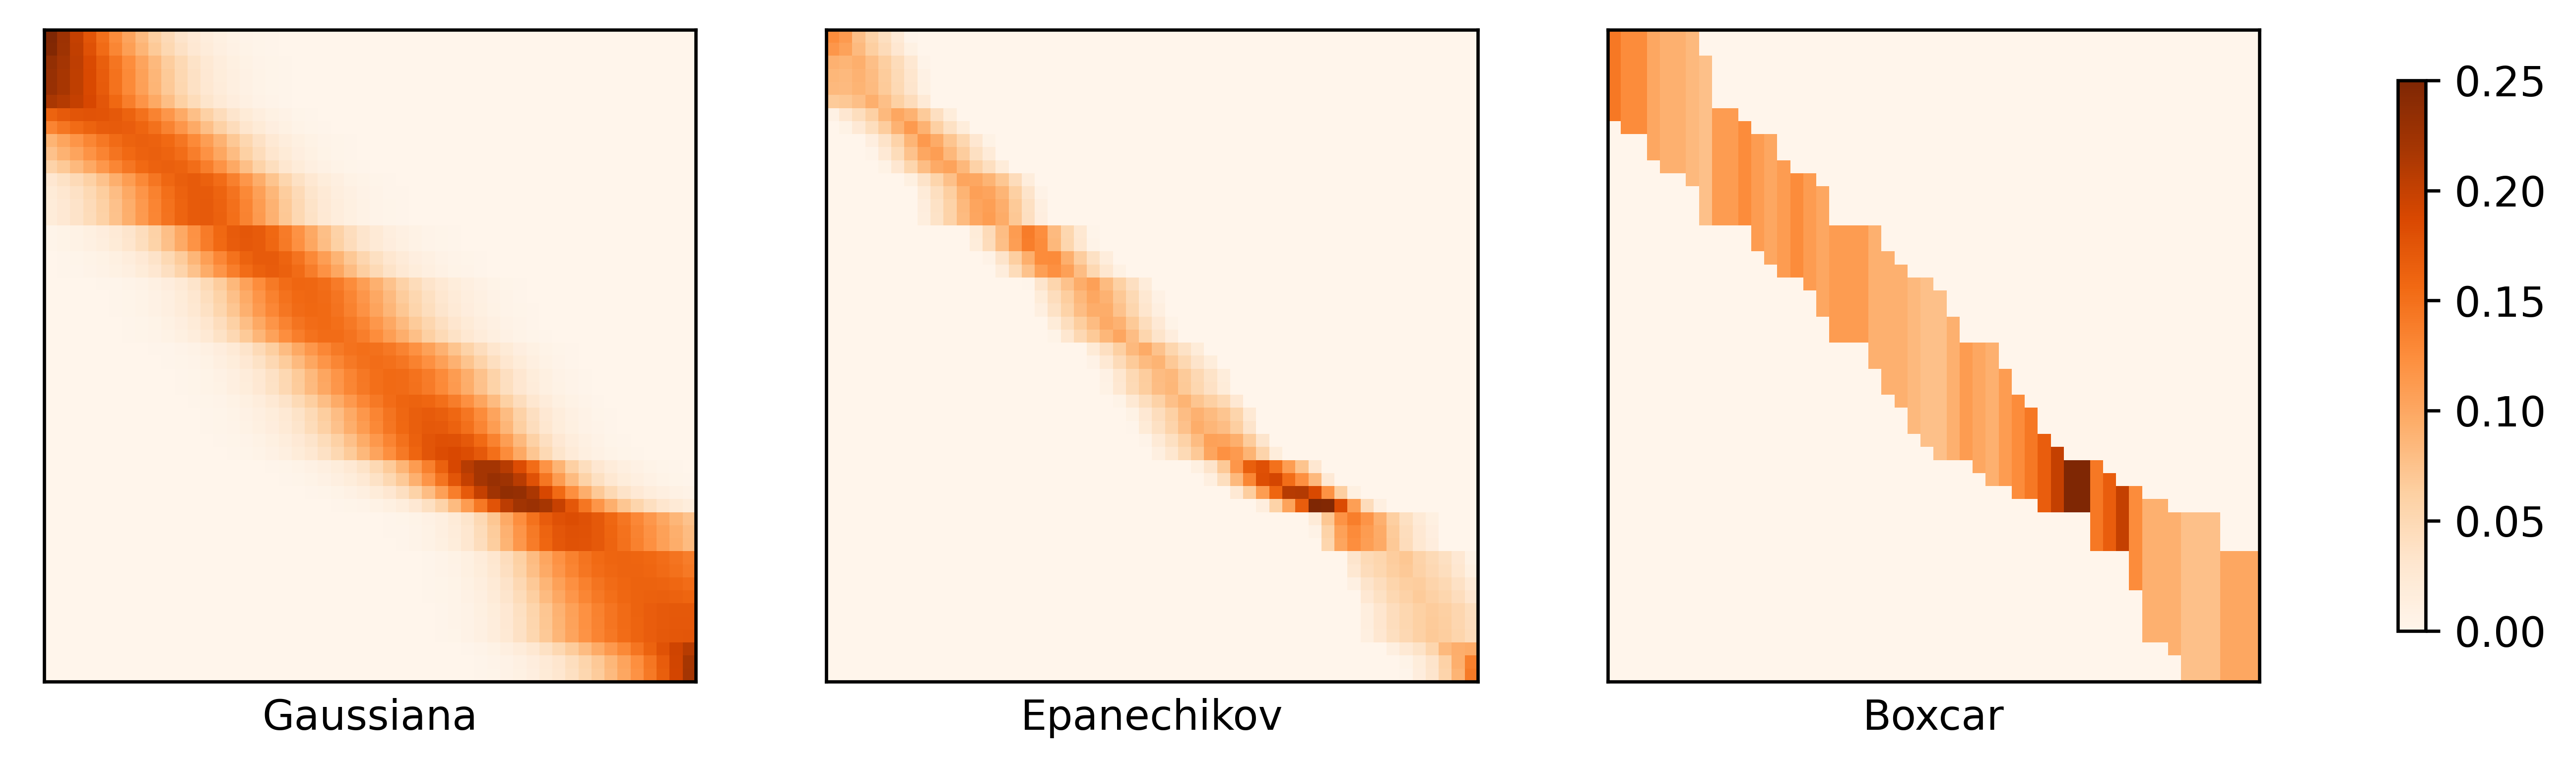
\includegraphics[width=\textwidth]{figures/chapter4/heatmap.png}
    \caption{Visualización de los \textit{pesos de atención}. Se trata de la representación de la matriz \( M \) tal que \( M_{ij} = \alpha(x^\text{val}_{i}, x_j) \), donde el color representa la magnitud de la componente.}
    \label{fig:kernel}
\end{figure}

El estudio del estimador de Nadaraya-Watson cumple un triple propósito: en primer lugar, muestra la flexibilidad de los métodos de atención y su relación con métodos clásicos de inferencia estadística. En segundo lugar, sirve para exhibir una de los grandes atributos de los métodos de atención: la posibilidad de visualizar los pesos de atención a fin de poder entender el funcionamiento del modelo. En tercer lugar, muestra lo decisivo de la elección de la representación de la base de datos (claves y valores). En última instancia, la complejidad de elegir representaciones adecuadas lleva a diseñar esta representación de forma que sea \textit{aprendida} como una parte más de los parámetros del modelo.

\section{Funciones de similitud}
Los mecanismos de atención son conceptualmente independientes de la función de similitud concreta escogida. Existen varias razones, no obstante, por las que merece la pena detenerse a estudiar algunas de las posibles funciones de similitud. En primer lugar, elegir una función de similitud es imprescindible para poder realizar un análisis riguroso de la complejidad computacional asintótica de la operación de atención. En segundo lugar, la elección de una buena función de similitud es una condición imprescindible para que la atención pueda ser utilizada para resolver problemas.

La función de similitud dominante es el \textit{producto escalar normalizado}. Partamos del caso en el que tenemos una serie de consultas \( \Set{ q_1, …, q_N} \) y una base de datos \( \mathcal{D} = \Set{(k_n, v_n)}_{n = 1}^N \) de forma que consultas, claves y valores pertenecen al mismo espacio vectorial. Consideremos el logaritmo del \textit{kernel} de atención Gaussiano para una consulta \( q \) y una clave \( k_{n} \):
\[
    a(q, k_n) = -\frac{1}{2} \|q - k_n\|^2  = q^T k - \frac{1}{2} \| k_n \|^2 - \frac{1}{2} \| q \|^2
\]

Las redes neuronales contemporáneas están severamente normalizadas, lo que permite omitir el último término, que solo depende de \( q \). También el penúltimo término puede eliminarse sin demasiada repercusión, pues la normalización de la red asegurará que la norma \( \| k_n \| \) de todas las claves será aproximadamente constante.

La función de producto escalar normalizado se obtiene normalizando el resultado, de forma que si suponemos que \( q, k \in \real{d} \) son vectores independientes e idénticamente distribuidos con media \( 0 \) y varianza \( 1 \) el \textit{kernel} también tenga media \( 0 \) y varianza \( 1 \).

\begin{definition}[Producto escalar normalizado]
Dada una consulta \( q \in \real{d}\) y un conjunto de claves \( \Set{k_n}_{n = 1}^N \) con \( k_n \in \real{d} \) definimos la función de similitud de producto escalar normalizado como:
\[
    \alpha_\text{dot}(q, k_{n}) = \frac{\exp \left\{q^t k_{n} / \sqrt{d} \right\}}{\sum_j \exp \left\{ q^t k_{j}/\sqrt{d} \right\}}
\]\
\end{definition}

Esta función de atención tiene excelentes propiedades computacionales pues si agrupamos las consultas, claves y valores en matrices \( Q = [q_1, …, q_{M}], K = [k_1, …, k_N], V = [v_1, …, v_N] \) entonces:
\begin{equation} \label{eq:dot_product}
    \attention(q_i, \Set{(k_{n}, v_{n})}; \alpha_\text{dot}) = V \softmax \left( \frac{K^T Q}{\sqrt{d}} \right) e_i
\end{equation}
siendo:
\[
    \softmax \left( A \right)_{ij} \equiv \frac{\exp \left\{ A_{ij} \right\}}{\sum_k \exp \left\{ A_{kj} \right\}}
\]
expresión que puede calcularse de forma extremadamente eficiente.

El problema de la expresión en la \cref{eq:dot_product} es que puede que no queramos que todas las consultas se calculen sobre la misma base de datos. Este problema puede resolverse de forma computacionalmente eficiente utilizando una \textit{máscara}:
\begin{definition}[Atención con máscara]
    Dadas matrices \( Q \in \real{d_\text{attn} \times d_q}\), \(K \in \real{d_\text{attn} \times d_k}\), \(V \in \real{d_\text{attn} \times d_v}\) y una máscara \( \mathcal{M} \in \Set{0, 1}^{d_k \times d_q}\) llamamos \textit{atención con máscara} o \textit{masked attention} a la función:
    \begin{align*}
        \mattention(Q, \mathcal{D}, \mathcal{M}) = V\softmax(S/\sqrt{d}) && S_{ij} = \begin{cases}
            (K^TQ)_{ij} & \text{si $\mathcal{M}_{ij} = 1$} \\
            -\infty & \text{si $\mathcal{M}_{ij} = 0$} 
        \end{cases}
    \end{align*}
\end{definition}


\section{Atención multicabezal (\textit{multihead})}
En los modelos diseñados para el procesamiento de lenguaje natural, las consultas y la base de datos se construyen como proyecciones de los símbolos de entrada (una vez \textit{tokenizados}). En ese caso, las consultas y la base de datos pueden presentar relaciones tan complejas como los datos en sí mismos y el uso directo del mecanismo de atención resulta demasiado restrictivo.

Se introduce para ello una variante de la atención llamada \textit{atención multicabezal}, que parte de la idea de crear distintos \textit{cabezales} de atención cada uno de los cuales trabaje con proyecciones distintas de la base de datos. Formalizamos esta idea:

\begin{definition}[Cabezal de atención (\textit{attention head})]\label{eq:attention_head}
    Sea \( q \in \real{d_q} \) una consulta, y \( \mathcal{D} = \Set{(k_n, v_n)}_{n = 1}^N \) con \( k_n \in \real{d_k}, v_n\in \real{d_v} \) una base de datos. Sean \( p_q, p_k, p_v \in \nat \) y \( \alpha \colon \real{p_q} \times \real{p_k} \to \realo \) una función de similitud. Dadas matrices \( W^q \in \real{p_q \times d_q}, W^k \in \real{p_k \times d_k}, W^v \in \real{p_v \times d_v} \) definimos un cabezal de atención \( H \) como la función:
    \begin{equation} \label{eq:head}
        \head(q, \mathcal{D}; W^q, W^k, W^v, \alpha)  = \attention(W^q q, \Set{(W^k k_n,  W^v v_n)}; \alpha)
    \end{equation}
\end{definition}

Al combinar los cabezales de atención se obtiene una \textit{atención multicabezal}
\begin{definition}[Atención multicabezal (\textit{multihead attention})]     
     Sean \( (\head_{i})_{i = 1}^{n_h} \) cabezales de atención con parámetros \( \theta_{i} = \Set{ W^q_{i}, W^k_{i}, W^v_{i} } \). Dado \( p_o \in \nat \) y una matriz \( W^o \in \real{p_0 \times n_h p_v} \) definimos la atención multicabezal como la función:
     \[
        \multihead \left(q, \mathcal{D}; \mathfrak{W}, \alpha \right) = W^o \begin{pmatrix} \head_{1}(q, \mathcal{D}; \theta_{1}, \alpha) \\ \vdots \\ \head_{n_h}(q, \mathcal{D}; \theta_{n_h}, \alpha) \end{pmatrix}
     \]
     con \( \mathfrak{W} = \bigcup_i \theta_i \cup \Set{W^o} \).\footnote{En la línea de la \cref{eq:dot_product}, dadas matrices \( Q = [q_1, …, q_{n_q}], K = [k_1, …, k_n], V = [v_1, …, v_n] \) resulta práctico introducir la notación \( \multihead(Q, K, V) \), definida como la matriz que tiene por columna i-ésima \( \multihead(q_i, \Set{(k_n, v_n)}) \). Utilizaremos esta notación al estudiar cómo implementar la arquitectura \textit{transformer}.}
\end{definition}

La definición anterior proporciona una forma directa de definir la capa de atención, como la capa que computa la función \( \multihead \) para una elección concreta de \( \alpha \), de forma que todas las matrices \( W \) son proyecciones aprendidas por la red. 

Habitualmente, \( \alpha \) es la función de producto escalar normalizado, lo que hace directo definir una variante de la atención multicabezal con máscara utilizando cabezales que usen la atención con máscara, que denotaremos \( \mmultihead(\smallbullet, \mathcal{M}; \mathfrak{W}) \). 

La investigación ha demostrado que la atención multicabezal es una técnica muy efectiva: durante el entrenamiento se desarrollan cabezales especializados con una función interpretable \cite{voita2019analyzing}. En el caso del lenguaje natural, por ejemplo, se han identificado cabezales con una función \textit{posicional}, \textit{sintáctica} y para la identificación de \textit{términos infrecuentes}.

Otra ventaja de la atención multicabezal proviene de que usualmente la dimensión del espacio de proyección es considerablemente menor que la dimensión original de las consultas y la base de datos. Dado que los cálculos en los distintos cabezales son paralelizables, la atención multicabezal permite reducir el tiempo necesario para el cálculo de la atención. Estudiaremos con más detenimiento este punto cuando analizemos la complejidad computacional asintótica de los mecanismos de atención.

\section{Complejidad computacional asintótica de la atención}
Presentadas ya las funciones de similitud más habituales, emprendemos el estudio de la complejidad computacional asintótica de los mecanismos de atención. Asumiremos que utilizamos el producto escalar como función de similitud y que las consultas, claves y valores están representados por matrices de dimensión \( d \times n \).

Para calcular la atención comenzamos proyectando las consultas, claves y valores mediante la multiplicación por matrices de proyección aprendidas \( W^q \in \real{d_q \times d}, W^k \in \real{d_q \times d}, W^v \in \real{d_v \times d}\), como se describe en la \cref{eq:attention_head}. Estas operaciones tienen un coste asintótico en \( \mathcal{O}((d_q + d_v)dn) \).

El cómputo de la atención requiere las siguientes operaciones: \begin{enumerate*}[label=(\roman*)]
    \item cálculo de \( K^T Q / \sqrt{d_k} \), que puede hacerse en tiempo \( \mathcal{O}(n^2 d_k) \)
    \item cálculo de la operación \( \softmax \), que puede hacerse en tiempo \( \mathcal{O}(n^2) \)
    \item cálculo del producto con la matriz \( V \), que requiere tiempo \( \mathcal{O}(n^2 d_v) \)
\end{enumerate*}, con lo que tiene complejidad \( \mathcal{O}(n^2 (d_k + d_v)) \).

Si utilizamos atención multicabezal con \( H \) cabezales, las operaciones anteriores tienen que realizarse una vez por cada cabezal. Sin embargo, \( H \) es habitualmente una constante pequeña \cite{voita2019analyzing} y la existencia de múltiples cabezales permite reducir los valores \( d_k, d_v \) sin deteriorar el rendimiento, reduciendo así la carga computacional de utilizar la atención multicabezal.

Una de las grandes ventajas del mecanismo de atención es que el cálculo de la atención para cada consulta es independiente del resto, lo que significa que su cálculo puede paralelizarse. De hecho, paralelizando los cálculos sobre cada cabezal y las multiplicaciones matriciales es posible realizar los cálculos con \( \mathcal{O}(1) \) operaciones secuenciales, teniendo el camino más largo también  \( \mathcal{O}(1) \) operaciones. 

La mayor debilidad computacional del mecanismo de atención proviene de la dependencia cuadrática sobre \( n \), el número de consultas, claves y valores. Dado que el tamaño de la base de datos y las consultas suele crecer linealmente con el tamaño de la secuencia de entrada, esto lo hace inviable para abordar problemas con secuencias de entrada muy largas.